\section{Cell assembly detection method}
\label{chap:AssemblyMethod}
\begin{framed}
On the described data-set I applied a cell-assembly detection method (CAD) developed in our lab (\cite{RussoDurstewitz}). In this section I present CAD to facilitate reading and interpretation of analysis results.\\The concept of cell-assembly was coined by Hebb (\cite{Hebb}), who described a cell-assembly as a group of neurons which, by functionally organizing into a temporally coherent set, come to represent mental or perceptual entities, thereby forming the basis of neural coding and computation. Nowadays the concept of cell-assembly is used loosely to describe a group of neurons that perform a given action or represent a given percept or concept in the brain. Thus the term cell assembly denotes in fact anything from the precise zero-phase-lag spike synchronization in a defined subset of neurons (\cite{Abeles}, \cite{Singer}, \cite{Roelfsema}, \cite{Diesmann}, \cite{Harris2003}) to temporally coherent changes in average firing rates on larger time scales (\cite{Goldman}, \cite{Durstewitz}) (\ref{fig:CellAsseDet}).
\begin{figure}[H]
    \centering
    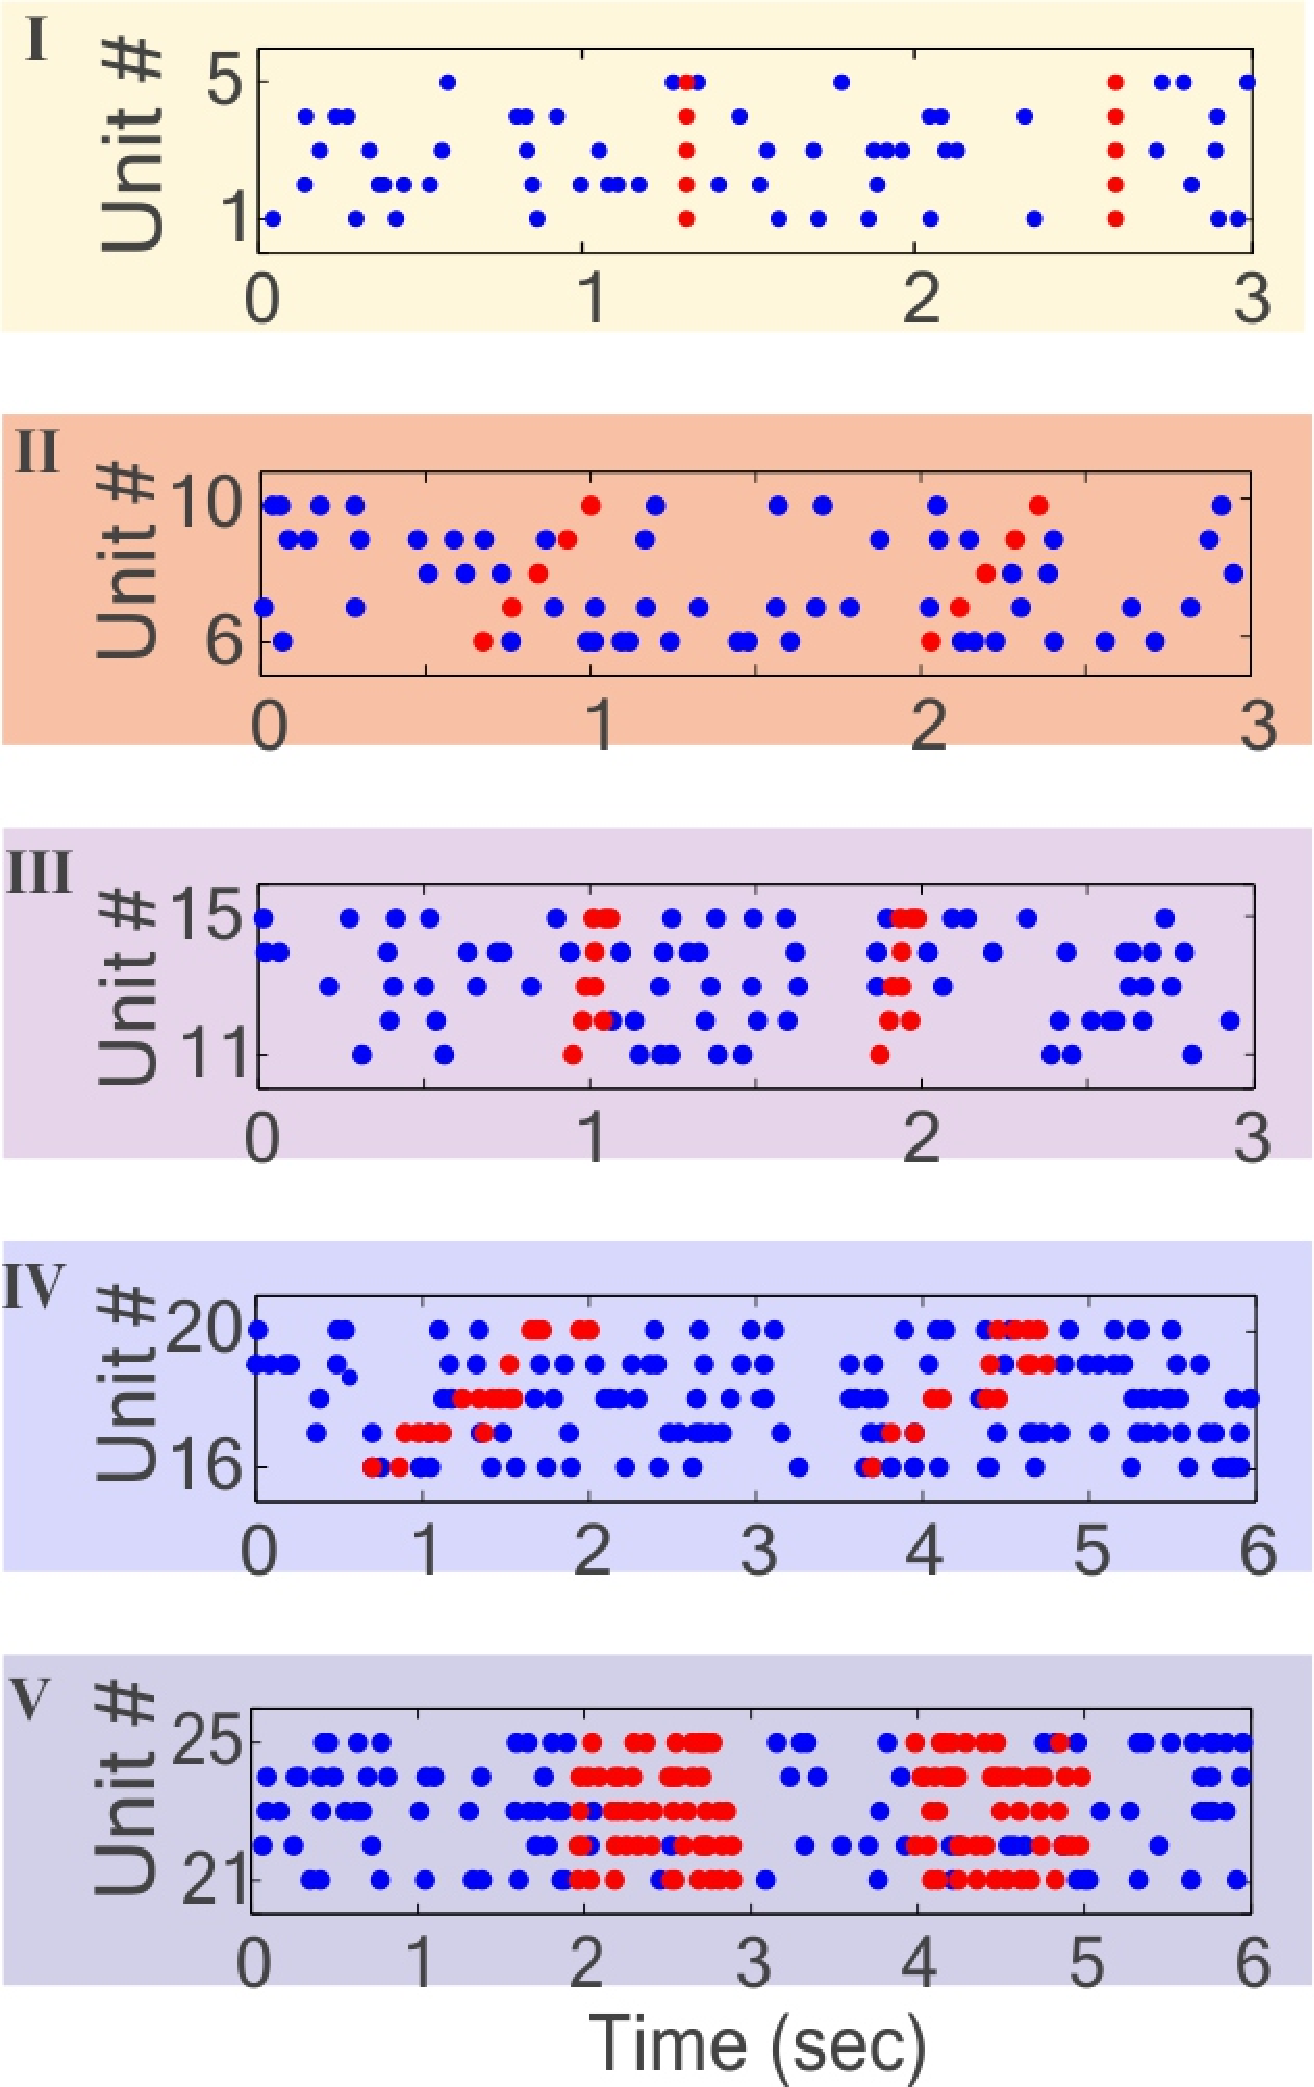
\includegraphics[scale=0.21]{figures/CellAssembliesZoom.pdf}
    \caption{Adapted from \cite{RussoDurstewitz}. Sketch of different types of cell assemblies differing in temporal precision and activity pattern.}
    \label{fig:CellAsseDet}
\end{figure}
In the recent years, neuroscientists have invested increasing efforts to understand how cell assemblies are formed and composed, to analyse their activation and their coding (\cite{Buzsaki1}, \cite{Liu}, \cite{Cai}). This increasing interest led to the development of numerous mining techniques for the detection and statistical testing of cell assemblies. However, because of the combinatorial explosion of the assembly patterns to test, most techniques limit the search for assembly patterns to one or the other assembly typology shown in figure \ref{fig:CellAsseDet} (\cite{Torre}, \cite{Tavoni}).\\CAD does not focus on a single specific assembly concept, theoretical idea, or particular time-scale. Instead it treats the temporal scale, precision, and internal organization of coherent activity patterns as free parameters, to be determined from the data, and is thus free to detect a large family of possible assembly definitions at any time scales and spike coordination.\\CAD is based on the idea that the activation of assembly occurs as repeating activity pattern in a the of simultaneously recorded spike trains. As shown in figure \ref{fig:CellAsseDet} a pattern of activity can be anything from a precise coordination of spikes to a broaden firing rate modulation, and from synchronous activation to an arbitrary distribution of lags between the activity of multiple units. The idea proposed with CAD is to capture the multiplicity of temporal scales and structures mentioned above and assess their statistical significance.\\At the first step, the algorithm detects and tests dependency between pairs of units, from which high order assemblies are recursively build up using an agglomerative procedure.\\Assume each recorded spike time series has been converted into a series $\{c_t\}$ of spike counts of length T at bin width $\Delta$, with $\#_A$ and $\#_B$ denoting the total numbers of spikes emitted by units A and B, respectively. In case of independence between A and B, the joint probability distribution of spike occurrences is the product of their marginal distributions, $p(A,B)=p(A)p(B)$.\\  If $\Delta$ is small enough such that $c_t\in\{0,1\}$ (binary counts), then, under the null hypothesis ($H_0$) of independence, the joint spike count $\#_{AB,l}$ at time lag $l$ follows a hypergeometric distribution with mean $\mu_{AB,l}=\#_A \#_B/(T-l)$ and variance $\sigma^{2}_{AB,l}$. If the binning is such that spike counts $c_t$ larger than one occur, the hypergeometric distribution is no longer directly applicable. In this case the series are split into several (mutually dependent) binary series for which it is still possible to derive a joint mean and variance (see Materials and Methods of \citeay{RussoDurstewitz}).\\It would be sufficient to use mean $\mu_{AB,l}$ and variance $\sigma^{2}_{AB,l}$ to check for deviation from the null hypothesis of independence $H_0$ at lag $l$, in practice such a statistic would be corrupted by non-stationarities (see Materials and Methods and Appendix of \cite{RussoDurstewitz}). Instead of using classical strategies for correcting non-stationarity such as sliding window (\cite{Gruen}) or bootstrap-based method (\cite{Fujisawa}, \cite{Pipa}, \cite{Picado}), which imply considerable computational burden, \citeay{RussoDurstewitz} alternatively suggest a new simple remedy for non-stationarity based on difference in counts $\#_{ABBA,l^-} \equiv \#_{AB,l^-} - \#_{AB,l^*}$ that subtracts from each joint spike count $\#_ {AB,l^-}$ the number $\#_{AB,l^*}$ of occurrences of the reference pattern $(A,B)_{l^*}$. The statistic $Q_{AB,l}\equiv\#_{ABBA,l^2}/\hat{\sigma}_{ABBA}^2$ is approximately F-distributed and can be used for fast parametric assessment of the null hypothesis. It is important to notice that the difference statistic corrects for non-stationarity artifacts and, because parametric, limits the computational load. This permits to test multiple bin sizes. The whole procedure is repeated for a set of user-defined bin widths $\Delta \in \{\Delta_{min},...,\Delta_{max}\}$. For each formed assembly, the width $\Delta^*$ associated with the lowest p-value is defined as its temporal precision or its typical time scale.\\CAD is particularly suited to investigate neural VS-VTA interaction in dynamic tasks such as reinforcement learning. In fact, reversal learning tasks are highly dynamic, requiring quick changes in the network state. Such strong non-stationarity, if not accounted for as done in CAD can lead to an high false discovery rate, compromising the correct interpretation of VS-VTA interactions. Moreover, whilst other methods often propose to detect cell assemblies by aligning the population activity to task/behavioral events, CAD sums evidence of assembly activity throughout the task and session. This makes possible the detection of the same assembly even if its time of activation changes within the trial.
\end{framed}
